%!TeX spellcheck = en-GB

\documentclass[hyperref={colorlinks=true,urlcolor=blue,linkcolor=.},aspectratio=1610,mathserif]{beamer}
\usepackage[utf8]{inputenc}
\usepackage{pgfpages}
\usepackage{graphicx}
\usepackage{pdfpages}
\usepackage{tikz}
\usepackage[many]{tcolorbox}
\usepackage[autoplay,loop,keepaspectratio]{animate}
\usepackage{siunitx}
\sisetup{
	per-mode = power,
	round-mode = figures,
	round-precision = 3,
	scientific-notation = false,
	output-decimal-marker = {.},
	exponent-product = \times,
	separate-uncertainty = true,
	uncertainty-separator = ,
	output-product = \cdot,
	quotient-mode = fraction,
	range-phrase = -,
	range-units = single,
	inter-unit-product = \ensuremath{{\cdot{}}},
	number-unit-product = \,,
	multi-part-units = single,
	alsoload = synchem,
}
\DeclareSIUnit\atm{atm}
\usepackage{nth}
\usepackage{physics}
\usepackage{pgfplots}
\pgfplotsset{width=10cm}
\def\axisdefaultwidth{10cm}
%\usepgfplotslibrary{external}
\usepgfplotslibrary{units}
%\tikzexternalize

\usepackage{appendixnumberbeamer}
% Add total frame count to slides, optional. From Stefan,
% http://www.latex-community.org/forum/viewtopic.php?f=4&t=2173
\expandafter\def\expandafter\insertshorttitle\expandafter{%
  \insertshorttitle\hfill\insertframenumber\,/\,\inserttotalframenumber}

% ------------------------ Define note handout layout -------------------------
\newcommand{\pgflayout}{
	\pgfpagesphysicalpageoptions
	{%
		logical pages=2,%
		physical height=210mm,%
		physical width=297mm,%
	}%
	\pgfpageslogicalpageoptions{2}
	{%
		resized width=\pgfphysicalwidth,%
		resized height=\pgfphysicalheight,%
		center=\pgfpoint{.5\pgfphysicalwidth}{.25\pgfphysicalheight}%
	}%
	\pgfpageslogicalpageoptions{1}
	{%
		resized width=\pgfphysicalwidth,%
		resized height=\pgfphysicalheight,%
		center=\pgfpoint{.5\pgfphysicalwidth}{.70\pgfphysicalheight}%
	}%
}
% -----------------------------------------------------------------------------

% ---------------------------- Show note handout: -----------------------------
%\setbeameroption{show only notes}
%\pgflayout
% -----------------------------------------------------------------------------

% -------------------------- Define Beamer options ----------------------------
\beamertemplatenavigationsymbolsempty
\usefonttheme{serif}
\usecolortheme{beaver}

\setbeamertemplate{footline}
{%
	\begin{beamercolorbox}{section in foot}
		\begin{center}
			\vskip2pt\insertnavigation{\paperwidth}\vskip2pt
		\end{center}
	\end{beamercolorbox}%
}

\setbeamertemplate{note page}{%
	\vskip7em
	\begin{columns}[c]{\paperheight}
		\column{0.5\paperheight}
		\insertnote
		\column{0.5\paperheight}
		\insertslideintonotes{0.5}
	\end{columns}%
}

\setbeamersize{text margin left=30mm,text margin right=30mm}

\definecolor{DTUred}{cmyk}{0,0.91,0.72,0.23}
\definecolor{itemcolor}{cmyk}{0,0,0,0.56}
\definecolor{blockbodycolor}{cmyk}{0,1,1,0.5}
\definecolor{White}{cmyk}{0,0,0,0}
\setbeamercolor{titlelike}{fg=DTUred}
\setbeamercolor{section in head/foot}{fg=DTUred}
\setbeamercolor{section in toc}{fg=DTUred}
\setbeamercolor{itemize item}{fg=itemcolor}
\setbeamercolor{redbox}{fg=White,bg=blockbodycolor}
\setbeamercolor{description item}{fg=DTUred}
% -----------------------------------------------------------------------------

\title{Exam presentation}
\subtitle{Course 10401}
\author{\scshape\centering Rasmus Kronborg Finnemann Wiuff (s163977) \\ \vspace{7.5mm} 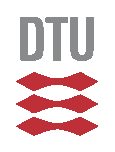
\includegraphics[width=1cm]{Figures/DTU3CMYK.eps}}
\date{\scshape January 17, 2019}

\begin{document}

\begin{frame}[plain]
	\titlepage
\end{frame}

\section{Introduction}
\subsection{Introduction}
\begin{frame}{Introduction}
	\begin{center}
		\begin{columns}[t]
			\column{.7\textwidth}
			\textbf{DTU Tokamak Interferometer}\newline
			\vspace{.26em}
			\begin{description}[Goal \# 1]
				\item[Title] Diagnostics via interferometry
				\item[Goal \# 1] To calculate the phase shift induced by O-mode plasma and investigate different microwave sources
				\item[Goal \# 2] To design a lens system to accommodate the beam propagation in the small DTU tokamak
			\end{description}
			\column{.7\textwidth}
			\textbf{Fusor Spectral Lines}\newline
			\begin{description}[Goal \# 1]
				\item[Title] Fusor exercise
				\item[Goal \# 1] To measure spectral lines from fusion in the inertial electrostatic confinement fusor at DTU
				\item[Goal \# 2] To estimate velocities and energies as functions of voltage
			\end{description}
		\end{columns}
	\end{center}
\end{frame}

\section{Plasma Interferometry}
\subsection{Cut off/sources}
\begin{frame}{Cut off}
	\centering
	\begin{align}
		\qq{Proportionallity:} \omega_p^2    & \propto n_\mathrm{e}                   \\
		\qq{Refreactive index:} N_\mathrm{O} & = \sqrt{1-\frac{\omega_p^2}{\omega^2}}
	\end{align}
	The plasma is transparent if
	\begin{align}
		\omega > \omega_p = \sqrt{n_\mathrm{e}\frac{e^2}{\varepsilon_0m_\mathrm{e0}}}
	\end{align}
	For \(\omega\), \(n_\mathrm{e}\) must not exceed cutoff density \(n_\mathrm{c}\):
	\begin{align}
		n_\mathrm{e} < n_\mathrm{c} & = \omega^2\frac{\varepsilon_0m_\mathrm{e0}}{e^2}                                                        \\
		n_\mathrm{c}                & = \omega^2\frac{\SI{8.854e-12}{\farad\per\meter}\ \SI{9.109e-31}{\kilo\gram}}{\SI{1.602e-19}{\coulomb}}
	\end{align}
\end{frame}

\begin{frame}{Cut off}
	\centering
	\begin{align}
		n_\mathrm{e} < 0.000314\omega^2
	\end{align}
	Electron density range: \SIrange{e16}{e18}{\per\meter\cubed}
	\begin{align}
		\omega & > \sqrt{\frac{\SI{e18}{\per\meter\cubed}}{0.000314}} \\
		       & \Downarrow\nonumber                                  \\
		f      & \approx \SI{9}{\giga\hertz}
	\end{align}
\end{frame}
\begin{frame}{Four Sources}
	\begin{columns}
		\column{.6\textwidth}\\
		At a density of \SI{e18}{\per\meter\cubed} the minimum frequency of the wave is:
		\(f \approx \SI{9}{\giga\hertz}\)\newline
		\begin{itemize}
			\item \SI{2.45}{\giga\hertz}
			\item \SI{60}{\giga\hertz} (Transparent)
			\item \SI{98}{\giga\hertz} (Transparent)
			\item \SI{130}{\giga\hertz} (Transparent)
		\end{itemize}
		\column{.6\textwidth}
		\includegraphics[width=\textwidth]{Figures/BeamProp.eps}
	\end{columns}
\end{frame}
\begin{frame}{Phase shift}
	\centering
	\begin{align}
		N_\mathrm{O} = \sqrt{1-\frac{\omega_p^2}{\omega^2}} = \sqrt{1-\frac{n_\mathrm{e}}{n_\mathrm{c}}}
	\end{align}
	Probing frequency much higher than plasma frequency, critical density much higher than electron density:
	\begin{align}
		N_\mathrm{O} & = \sqrt{1-\frac{n_\mathrm{e}}{n_\mathrm{c}}}         \\
		             & \approx 1-\frac{1}{2}\frac{n_\mathrm{e}}{\mathrm{c}} \\
		             & = 1-\frac{\omega_p^2}{2\omega^2}
	\end{align}
	% O-mode refractive index and electron density linear dependent if:
	% \begin{align}
	% 	\frac{n_\mathrm{e}}{n_\mathrm{c}} \leq0.4 \quad \frac{\omega_p}{\omega}           \leq0.6
	% \end{align}
\end{frame}

\begin{frame}{Phase shift}
	The phase shift is given as:
	\begin{align}
		\frac{\Phi}{2\pi} & = \frac{\Delta L_{opt}}{\lambda} = \frac{\int_{x_1}^{x_2}\pqty{N_V-N_{\mathrm{O}}(x')}\dd{x'}}{\lambda} \approx \frac{1}{2\lambda n_c}\int_{0}^{x}n_\mathrm{e}(x')\dd{x'} \nonumber \\
		                  & = 4.48\times 10^{-16} \pqty{\frac{\lambda}{\si{\meter}}}\int_{0}^{x}\pqty{\frac{n_\mathrm{e}(x')}{\si{\per\meter\cubed}}}\pqty{\frac{\dd{x'}}{\si{\meter}}}
	\end{align}
	Assuming a Gaussian density distribution:
	\begin{align}
		\int_{-\infty}^{\infty}n_\mathrm{e} \exp\pqty{-\frac{(y-b)^2}{2c^2}}\dd{y} \approx n_\mathrm{e}\ c\ \sqrt{2\pi}
	\end{align}
	With tokamak diameter of \SI{0.250}{\meter}:
	\begin{align}
		\frac{\Phi}{2\pi} & \approx 4.48\times 10^{-16}\pqty{\frac{\lambda}{\si{\meter}}}n_e\SI{0.25}{\meter}\sqrt{2\pi}                                          \\
		                  & = 1.12\times 10^{-16}\ n_e  \pqty{\frac{\sqrt{2\pi} c}{\omega\si{\meter}}} = 8.416\times 10^{-8}\pqty{\frac{n_e}{\omega\si{\second}}}
	\end{align}
\end{frame}

\begin{frame}{Phase shifts}
	\includegraphics[width=.9\textwidth]{MatlabFigures/PhaseShift/PhaseShift.eps}
\end{frame}

\subsection{Gaussian telescope}
\begin{frame}{Beam waist propagation}
	\centering
	Beam Waist:
	\begin{align}
		w(z) = w_0(z)\sqrt{1+\pqty{\frac{\lambda z}{\pi w_0^2}}^2}
	\end{align}
	\begin{columns}[c]
		\column{.7\textwidth}
		\centering
		\includegraphics[width=.7\textwidth]{Figures/PropEx.eps}
		\column{.7\textwidth}
		\centering
		\includegraphics[width=.7\textwidth]{Figures/BeamProp.eps}
	\end{columns}
\end{frame}

\begin{frame}{Designing a Gaussian telescope Interferometer}
	\begin{align}
		d   & = f_0 + f_1                                                                                    \\
		w_2 & = \frac{f_1}{f_0}w_0                                                                           \\
		d_3 & = \frac{f_1}{f_0}\pqty{f_0+f_1-\frac{f_1}{f_0}d_0}                                             \\
		w_1 & = \frac{\lambda f_0}{\pi w_0}                                                                  \\
		d_1 & = \pqty{\frac{\frac{d_0}{f_0}-1}{\frac{w_0^2\pi}{f_0\lambda}+\pqty{\frac{d_0}{f_0}-1}^2}+1}f_0 \\
		d_2 & = d-d_1
	\end{align}
\end{frame}

\begin{frame}{Gaussian Telescope}
	\begin{columns}
		\column{.6\textwidth}
		\begin{itemize}
			\item Input parameters:\\
			      \(r_p = \SI{0.055}{\meter}\), \(r = \SI{0.125}{\meter}\),
			      \(w_0 = \SI{0.0275}{\meter}\), \(\mathrm{freq} = \SI{60}{\giga\hertz}\), \(d_0 = \SI{0.2}{\meter}\), \(d_r = \SI{0.1}{\meter}\), \(f_0 = \SI{0.25}{\meter}\), \(f_1 = \SI{0.2}{\meter}\)
			\item Output distances:\\
			      \(d_1 = \SI{0.224}{\meter}\), \(d_2 = \SI{0.226}{\meter}\), \(d_3 = \SI{0.232}{\meter}\)
			\item Output beamwaists:\\
			      \(w_1 = \SI{0.0145}{\meter}\), \(w_2 = \SI{0.022}{\meter}\)
			\item Wavelenght: \(\lambda = \SI{0.005}{\meter}\)
		\end{itemize}
		\column{.7\textwidth}
		\includegraphics[width=\textwidth]{MatlabFigures/Interferometer/Interferometer.eps}
	\end{columns}
\end{frame}

\begin{frame}{Beware}
	\centering
	\includegraphics[width=\textwidth]{Figures/Refraction.eps}
\end{frame}

\section{Fusor Exercise}

\begin{frame}{Spectrum}
	\begin{figure}[H]
		\centering
		\resizebox{\textwidth}{!}{
			\begin{tikzpicture}
				\begin{axis}[
						width=\textwidth,
						height=.8\textheight,
						title={Spectrum of light from fusion in the fusor},
						use units,
						x unit prefix=n, x unit=m,
						y unit=A.U.,
						xlabel=Wavelength,
						ylabel=Intensity,
						ymajorgrids=true,
						grid style=dashed,
						%scaled y ticks=manual:{\(10^{-9}\)}{\pgfmathparse{#1*10^9}}
					]
					\addplot[color=red] table {Data/SpectrumData.txt};
				\end{axis}
			\end{tikzpicture}
		}
	\end{figure}
\end{frame}

\begin{frame}{Spectral line width as function of applied voltage}
	\centering
	\includegraphics[width=.9\textwidth]{MatlabFigures/Asign3/VSigma.eps}
\end{frame}

\begin{frame}{Energy and velocity}
	Spectral line width:
	\begin{align}
		\sigma & = \Delta\lambda = \frac{\lambda_0}{c} v_\mathrm{1D} \\
		       & = \frac{\lambda_0}{c}\frac{kT}{m}^{1/2}
	\end{align}
	Kinetic energy:
	\begin{align}
		\mathrm{KE} = \frac{1}{2}mv^2
	\end{align}
\end{frame}

\begin{frame}{Energy and velocity}
	\centering
	\includegraphics[width=\textwidth]{MatlabFigures/Asign3/KineticVelo.eps}
\end{frame}

\section*{Questions}
\title{Questions}
\subtitle{}
\begin{frame}
	\titlepage
\end{frame}

\appendix
\section{Energy and velocity fits}
\begin{frame}{Energy and velocity fits}
	\begin{align}
		\qq{Velocity for hydrogen:}        & v = 3.12\times10^4 \sqrt{x}+1.72\times10^5   \nonumber \\
		\qq{Velocity for deuterium:}       & v = 0.7666\times10^4\sqrt{x}+2.295\times10^5 \nonumber \\
		\qq{Kinetic energy for hydrogen:}  & KE = 11.7x+287.7                             \nonumber \\
		\qq{Kinetic energy for deuterium:} & KE = 4.387x+637.3 \nonumber
	\end{align}
\end{frame}

\end{document}
